\section{System Model and Service Pipeline}\label{sec:requirements}
Big data is highly dependent on cloud-edge computing, which makes extensive use of multitenancy.
Multitenancy permits sharing one instance of infrastructures, platforms or applications by multiple tenants to optimize costs. This leads to common scenarios where a service provider offers subscription-based analytics capabilities in the cloud, or a single data lake is accessed by multiple customers. Big data pipelines then mix data and services which belong to various organizations, posing a serious risk of potential privacy and security violations.

We propose a data governance framework tailored to contemporary data-driven pipelines, which aims to limit the privacy and security risk. The primary objective of this framework is to facilitate the assembly of data processing services, with a central focus on the selection of those services that optimize data quality, while upholding privacy and security requirements.

In the following of this section, we present our system model (Section \ref{sec:systemmodel}) and our reference scenario (Section \ref{sec:reference}).

\subsection{System Model}\label{sec:systemmodel}
In today's data landscape, the coexistence of data quality and data privacy is critical to support high-value services and pipelines. The increase in data production, collection, and usage has led to a split in scientific research priorities.
%This has resulted in two main focus areas.
First, researchers are exploring methods to optimize valuable data. Here, ensuring data quality is vital, and requires accuracy, reliability, and soundness for analytical purposes.
Second, there is a need to prioritize data privacy and security. This involves safeguarding confidential information and complying with strict privacy regulations. These two directions are happening at the same time, but there are not many solutions that find a good balance between them.

Our approach seeks to harmonize these objectives by establishing a data governance framework that balances privacy and data quality. It implements a system model that is composed of the following parties:
\begin{description}
  \item[Service,] a software distributed by a \textbf{service provider} that performs a specific task according to access control privileges on data; %, a service can be tagged with some policies %, a service is characterized by two function: the service function and the policy function.
  \item[Pipeline,] a sequence of connected services that collect, prepare, process, and analyze data in a structured and automated manner. We distinguish between a \textbf{pipeline template} that acts as a skeleton, specifying the structure of the pipeline and the (non-)functional requirements driving  service selection, and a \textbf{pipeline instance} instantiating the template with services according to the specified requirements;
    \item[Data Governance Policy], a structured set of confidentiality guidelines, rules, and procedures regulating data access and protection;
  \item[User] that executes an analytics pipeline on the data. We assume that data target of the analytics pipeline are ready for analysis, that is, they underwent a preparatory phase addressing issues such as missing values, outliers, and formatting discrepancies. This ensures that the data are in an optimal state for subsequent analysis.
\end{description}

The \user starts its analytics by first selecting a pipeline template among a set of functionally-equivalent templates. The template is selected according to the \user\ non-functional requirements and then instantiated in a pipeline instance. In particular, for each component service in the template, a real service is selected among a list of candidate services in the instance. Candidate services are functionally equivalent and comply with the privacy policies specified in the template.
Candidate services are ranked based on their ability to retain the maximum amount of information (\emph{data quality} in this paper), while maintaining a minimum level of privacy.
%Priority is given to the service that maximizes data quality, while maintaining the same level of privacy. This evaluation process aids in identifying the most suitable service for a particular step in the pipeline.
Upon selecting the most suitable service for each component service in the pipeline template, the pipeline instance is completed and ready for execution.
%Our goal is not to formulate novel service composition algorithms, but rather to establish a data governance framework.

It is important to note that our data governance approach builds on the following assumption: \emph{upholding a larger quantity of data is linked to better data quality.} While this assumption is not true in all settings, it correctly represents many real-world scenarios. We leave a solution that departs from this assumption to our future work.
e
\subsection{Service Pipeline and Reference Scenario}\label{sec:service_definition}
We consider a service-based environment where a service pipeline is designed to analyze
data. We define a service pipeline as a graph defined as follows. % and depicted in \cref{fig:service_pipeline}.
\begin{definition}[\pipeline] \label{def:pipeline}
  A \pipeline is as a direct acyclic graph G(\V,\E), where \V\ is a set of vertices and \E\ is a set of edges connecting two vertices \vi{i},\vi{k}$\in$\V. The graph has a root \vi{r}$\in$\V, a vertex \vi{i}$\in$\V$_S$ for each service $s_i$, two additional vertices \vi{c},\vi{m}$\in$\V$_{\timesOperator}$$\subset$\V\ for each alternative ($\timesOperator$) structure modeling the alternative execution (\emph{choice}) of operations and the retrieval (\emph{merge}) of the results, respectively, and two additional vertices \vi{f},\vi{j}$\in$\V$_{\plusOperator}$$\subset$\V\ for each parallel ($\plusOperator$) structure modeling the contemporary execution (\emph{fork}) of operations and the integration (\emph{join}) of their results, respectively.
\end{definition}

We note that \{\vi{r}\}$\cup$\V$_S$$\cup$\V$_{\timesOperator}$$\cup$V$_{\plusOperator}$$=$\V, and \vi{c}, \vi{m}, \vi{f}, and \vi{j} model branching for alternative/parallel structures. We also note that root \vi{r} possibly represents the orchestrator.

% A service pipeline is as a direct acyclic graph G(\V,\E), where \V\ is a set of vertices, one for each service $s_i$ in the pipeline, \E\ is a set of edges connecting two services $s_i$ and $s_j$, and \myLambda\ is an annotation function that assigns a label \myLambda(\vi{i}), corresponding to a data transformation \F\ implemented by the service $s_i$, for each vertex \vi{i}$\in$\V.
Our reference scenario considers a service pipeline analyzing a dataset of individuals detained in Department of Correction facilities in the state of Connecticut while awaiting trial. In particular, the user, a member of the Connecticut Department of Correction (DOC), seeks to compare admission trends in Connecticut prisons with those in other US states.
The user's preferences align with a predefined pipeline template that orchestrates the following sequence of operations:
\emph{i)} Anonymization of the dataset.
\emph{ii)} Data enrichment, integrating data from the states of New York and New Hampshire.
\emph{iii)} Transformation of the dataset to derive state-specific data aggregations, including statistical measures like averages, medians, and clustering-based statistics.
\emph{iv)} Storage of the results in the corresponding states. Specifically, one copy remains in Connecticut (where sensitive information in the source dataset is not protected), while two additional copies are distributed to New York and New Hampshire (with sensitive information from the source dataset being safeguarded).

We note that the template requires the execution of the entire service within a single country. If the data needs to be transmitted beyond the boundaries of Connecticut, data protection measures must be implemented. A visual representation of the flow is presented in Figure \ref{fig:service_composition_example}.

\begin{figure}
  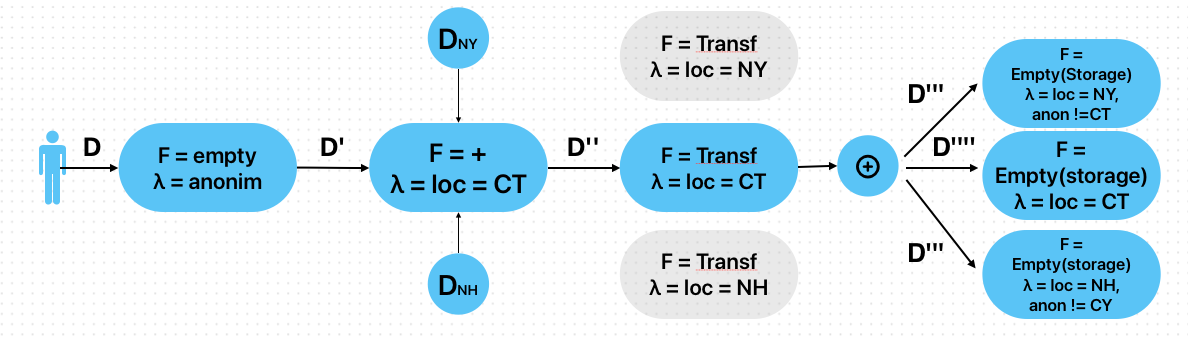
\includegraphics[width=0.98\columnwidth]{service_composition_example}
  \caption{Service composition example.}\label{fig:service_composition_example}

\end{figure}

The adopted dataset\footnote{https://data.ct.gov/Public-Safety/Accused-Pre-Trial-Inmates-in-Correctional-Faciliti/b674-jy6w} exhibits a straightforward row-and-column structure.
Each row represents an inmate; each column includes the following attributes: date of download, a unique identifier, last entry date, race, gender, age of the individual, the bound value, offense, entry facility, and detainer.
To serve the objectives of our study, we have extended this dataset by introducing randomly generated first and last names.


